\chapter{Background and Related Work}
\label{chap:background}

\section{Mental Health Monitoring and Wearable Sensing}

Mental health monitoring is difficult to perform continuously because many established assessment methods are episodic, retrospective, and dependent on active participation. Clinical interviews, questionnaires, and self-reports remain essential for diagnosis and care, but they usually capture a limited point in time rather than the continuous behavioral variation that occurs in everyday life. This limitation has motivated growing interest in wearable and mobile sensing as a complementary source of objective, timestamped data for mental-health-adjacent monitoring \cite{abdalrazaq2023wearable,gomes2023mentalhealth,levine2020passivesensing,lago2024longitudinal}.

Wearable devices are relevant in this context because they can collect signals during daily activity with relatively low user burden. Depending on the device, these signals may include motion, heart rate, sleep-related features, physiological variability, or other passive sensing streams. In this thesis, the focus is specifically on wrist-worn inertial measurement unit (IMU) data, especially accelerometer and gyroscope signals. Accelerometers capture linear acceleration and movement intensity, while gyroscopes capture angular velocity and rotational wrist motion. Together, these signals provide a practical basis for recognizing repeated hand and wrist movements that may be behaviorally relevant in anxiety- or stress-related contexts.

The mental-health relevance of wearable sensing must be framed carefully. Wearable data can support longitudinal observation and may reveal behavioral or physiological patterns that are difficult to capture through retrospective reports alone, but sensor data do not directly provide a clinical diagnosis. A smartwatch cannot infer anxiety, depression, or distress simply from motion signals without clinical context and validation. Therefore, this thesis treats wearable sensing as a support mechanism for mental-health-adjacent monitoring rather than as a diagnostic instrument.

This distinction is important for the thesis design. Instead of attempting to infer an internal mental state directly, the system operationalizes the monitoring problem through observable behaviors. Repetitive behaviors such as nail biting, hair pulling, hand scratching, hand tapping, and rubbing can appear in anxiety- or stress-related contexts and can also be represented as wrist-motion patterns. This makes the problem technically suitable for sensor-based Human Activity Recognition (HAR), while the broader application motivation remains continuous mental-health-adjacent monitoring.

The literature also shows that wearable mental-health monitoring is heterogeneous. Some studies focus on physiological anxiety or stress detection, some on mobile passive sensing, some on longitudinal symptom prediction, and others on behavior recognition from wearable motion signals \cite{abdalrazaq2023wearable,gomes2023mentalhealth,jacobson2021anxiety,levine2020passivesensing}. This heterogeneity is one reason why the scope of the present thesis is deliberately bounded. The thesis does not claim a clinically validated mental health monitoring system. It studies how wearable sensor data can be processed, monitored, and governed in an offline-first MLOps pipeline The literature also shows that wearable mental-health monitoring is heterogeneous. Some studies focus on physiological anxiety or stress detection, some on mobile passive sensing, some on longitudinal symptom prediction, and others on behavior recognition from wearable motion signals \cite{abdalrazaq2023wearable,gomes2023mentalhealth,jacobson2021anxiety,levine2020passivesensing}. This heterogeneity is one reason why the scope of the present thesis is deliberately bounded. The thesis does not claim a clinically validated mental health monitoring system. It studies how wearable sensor data can be processed, monitored, and governed in an offline-first MLOps pipeline when the observable task is anxiety-related behavior recognition.

Figure~\ref{fig:conceptual_framing} summarizes this bounded framing.

\begin{figure}[H]
    \centering
    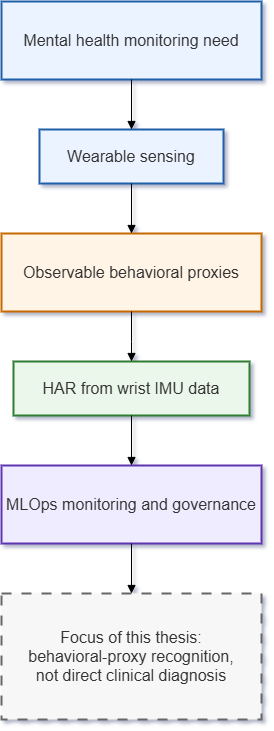
\includegraphics[width=0.70\textwidth,height=0.58\textheight,keepaspectratio]{figures/Figure_2_1_Conceptual_framing.png}
    \caption{Conceptual framing of wearable mental-health-adjacent monitoring in this thesis. The system uses wearable sensing to recognize observable behavioral proxies through HAR, rather than directly diagnosing mental health conditions.}
    \label{fig:conceptual_framing}
\end{figure}
\section{Anxiety-Related Behavioral Proxies and Human Activity Recognition}

The previous section established wearable sensing as a possible source of continuous mental-health-adjacent information. The next question is how this broad monitoring idea can be translated into a concrete machine learning task. In this thesis, the task is not direct mental-state inference. Instead, the monitoring problem is operationalized through observable anxiety-related behavioral proxies. These are externally visible behaviors that may appear in anxiety- or stress-related contexts, but they are not clinical labels by themselves.

Examples of such behaviors include nail biting, hair pulling, hand scratching, hand tapping, rubbing, and similar repetitive body-focused movements. These behaviors are relevant to this thesis because they are expressed through short, repeated wrist and hand motions. A wrist-worn IMU can capture part of this motion pattern through acceleration and angular velocity signals. Therefore, the technical problem can be framed as sensor-based Human Activity Recognition (HAR), where temporal windows of wearable sensor data are assigned to predefined activity classes \cite{lara2013survey,bulling2014tutorial,bao2004activity}.

This framing creates an important boundary. Recognizing a behavior is not the same as diagnosing anxiety. A model may classify a window as nail biting or hand tapping, but that prediction does not establish the user's mental state, the clinical meaning of the behavior, or the reason why the behavior occurred. The same behavior can appear in different contexts and can have different interpretations across individuals. For this reason, the behavioral labels used in this thesis are treated as activity labels, not as diagnostic labels.

Prior work supports the feasibility of recognizing anxiety-related or anxiety-displaying activities from wrist-worn motion signals. The ADAMSense study showed that activities such as nail biting, hair pulling, scratching, and tapping can be modeled from wearable sensor data using supervised learning \cite{khan2021adamsense}. The Garmin-based study used in this thesis context further shows that anxiety-related activities can be studied with commercial smartwatch sensor data and sequence-aware deep learning models \cite{oleh2025recognition}. These works justify the use of HAR as the recognition layer for the present thesis.

However, anxiety-related HAR is more difficult than coarse activity recognition such as walking, sitting, or standing. Many of the target activities are fine-grained, short, repetitive, and partially overlapping in their wrist-motion signatures. For example, hand scratching and rubbing may share similar gross movement intensity, while nail biting and hair pulling may depend on subtle wrist orientation and transition patterns. Recognition performance can therefore depend strongly on windowing, sensor placement, sampling rate, preprocessing, user movement style, and class definition.

This motivates the need for a pipeline view rather than a model-only view. If anxiety-related behaviors are represented as HAR classes, then the full runtime contract becomes important: the same sensor channels, unit conventions, preprocessing decisions, window size, stride, label order, and model input shape must be preserved during inference. A mismatch in any of these elements can change the meaning of the input window before the model makes a prediction. Therefore, the thesis treats behavioral-proxy recognition as both a HAR problem and an operational MLOps problem.

In summary, this thesis uses HAR as the technical bridge between wearable sensing and mental-health-adjacent monitoring. The behavioral proxy framing keeps the scope scientifically bounded: the system recognizes observable wrist-movement activities that may be relevant for later interpretation, but it does not infer clinical mental states directly. This distinction is central to the rest of the thesis, because it explains why the contribution focuses on reproducible sensing, inference, monitoring, and governance rather than on clinical diagnosis.

\section{Deep Learning for Wearable Sensor-Based HAR}

Wearable sensor-based HAR is commonly formulated as a multivariate time-series classification problem. Instead of classifying individual sensor samples, the continuous IMU stream is divided into temporal windows, and each window is assigned an activity label. This window-based representation is important because human activities are expressed through motion patterns over time rather than through isolated acceleration or gyroscope values. The choice of sampling rate, window length, overlap, and channel order therefore directly shapes the information available to the model \cite{lara2013survey,bulling2014tutorial,bao2004activity}.

Traditional HAR pipelines often used hand-crafted temporal and spectral features followed by classical classifiers. Deep learning changed this workflow by allowing models to learn representations directly from raw or lightly processed sensor windows. This is especially useful for wearable IMU data, where discriminative information may appear as local peaks, periodic patterns, temporal transitions, or combinations of acceleration and angular velocity across multiple axes \cite{wang2019sensorhar,zhang2022wearablehar,oleh2024harreview}.

Convolutional neural networks (CNNs) are useful in this setting because they can learn local temporal patterns from sensor windows. In one-dimensional sensor signals, 1D convolutions can capture short motion motifs such as repeated tapping, rubbing, or wrist rotations. Recurrent models, especially Long Short-Term Memory (LSTM) networks, are designed to model temporal dependencies across sequences \cite{hochreiter1997lstm}. Bidirectional LSTMs extend this idea by processing the sequence in both forward and backward directions, allowing the model to use temporal context from both sides of a window \cite{schuster1997bilstm}.

Hybrid CNN--LSTM architectures combine these strengths. The convolutional part extracts local motion features, while the recurrent part models their temporal ordering. Such combinations have been widely used in sensor-based HAR because they preserve both local movement structure and longer temporal dependencies \cite{ordonez2016deep,hammerla2016deep,lyons2021improved}. In time-series classification more generally, 1D-CNN models have also been shown to provide strong baselines when applied directly to raw temporal signals \cite{wang2017timeseries1dcnn}.

This model family is particularly relevant for anxiety-related wrist behavior recognition. Activities such as nail biting, hair pulling, hand scratching, and hand tapping are not always separable by movement intensity alone. They may require the model to capture short repeated motion motifs, rotational transitions, and temporal context within the window. Prior work on ADAMSense used deep sequence modeling for anxiety-displaying activities from wearable motion sensors \cite{khan2021adamsense}. The Garmin-based study used as a foundation for this thesis similarly applies a 1D-CNN-BiLSTM architecture to commercial smartwatch sensor data for anxiety-related activity recognition \cite{oleh2025recognition}.

However, deep learning does not remove the need for careful pipeline design. A deep model can learn useful representations only under the assumptions present during training. If the inference pipeline changes the units, sampling rate, channel order, scaler policy, window construction, or label mapping, the model may receive data that no longer matches its learned input contract. Therefore, in this thesis, the 1D-CNN-BiLSTM model is treated not as an isolated artifact but as one component of a larger runtime contract. The model, preprocessing configuration, scaler, baseline, and label order must remain consistent for the predictions to be meaningful.

The role of deep learning in this thesis is therefore bounded. The thesis does not claim to propose a new neural architecture. Instead, it uses a defensible HAR model family as the predictive component inside a reproducible MLOps pipeline. The main research focus is how such a model is operationalized, monitored, and governed under production-style wearable conditions where labels may be unavailable and train--serve assumptions may be fragile.

Figure~\ref{fig:deep_har_workflow} summarizes the generic deep HAR workflow used as the model basis in this thesis.

\begin{figure}[H]
    \centering
    \includegraphics[width=0.90\textwidth,height=0.42\textheight,keepaspectratio]{figures/Figure_2_2_Deep_HAR_workflow.png}
    \caption{Generic deep-learning workflow for wearable sensor-based HAR. Multichannel IMU windows are processed through local temporal feature extraction and sequence modeling before activity classification.}
    \label{fig:deep_har_workflow}
\end{figure}
\section{Datasets, Wearables, and Domain Shift}

Datasets strongly shape what a wearable HAR model can learn and how its results should be interpreted. Many established HAR datasets are collected under controlled or semi-controlled conditions, where participants perform predefined activities, sensors are placed according to a protocol, and labels are available for evaluation. Examples such as early accelerometer-based HAR datasets and benchmark datasets like UCI HAR and PAMAP2 helped standardize window-based activity recognition and made model comparison easier \cite{bao2004activity,uciHar2013,reiss2012pamap}. However, such datasets often differ from the conditions expected in continuous wearable monitoring, where users move naturally, sessions may be noisy, labels may be incomplete, and sensor placement can vary.

For anxiety-related behavior recognition, the dataset problem becomes more specific. The relevant activities are not only general activities such as walking, sitting, or standing, but fine-grained hand- and wrist-centered behaviors such as nail biting, hair pulling, hand scratching, hand tapping, rubbing, and related repetitive motions. The ADAMSense work is important because it directly studies anxiety-displaying activities using wearable motion sensors and provides evidence that such behaviors can be modeled as a supervised HAR task \cite{khan2021adamsense}. This makes it a close conceptual foundation for the present thesis.

At the same time, transferring this idea to a commercial smartwatch setting introduces a lab-to-life gap. Research datasets often use controlled collection protocols and may rely on specific sensor devices, placements, sampling rates, and preprocessing conventions. Commercial wearables, by contrast, are designed for everyday use and may expose data through device-specific APIs, sampling behavior, unit conventions, and firmware-dependent characteristics. A model that performs well in one sensor environment may therefore not behave the same way when applied to data from another device or user group.

The Garmin-based study used in this thesis context is especially relevant because it moves anxiety-related HAR toward a commercial smartwatch setting. It shows that a 1D-CNN-BiLSTM model can be adapted to Garmin Venu 3 sensor data for anxiety-related activity recognition \cite{oleh2025recognition}. This supports the feasibility of the thesis task, but it also highlights the engineering problem: the model is only meaningful when the runtime data preserve the expected sensor channels, units, sampling rate, preprocessing sequence, windowing logic, and label order.

Lab-to-life shift can appear in several ways. First, user variability affects how the same behavior is performed. Nail biting, rubbing, or tapping may differ in speed, intensity, duration, and wrist orientation across users. Second, sensor displacement can change the measured signal even when the activity is the same. Wrist-worn devices may rotate, loosen, or shift during use, and such displacement has been shown to affect HAR performance \cite{wang2024enhancing}. Third, device and preprocessing differences can create train--serve mismatch. A change in acceleration units, gyroscope units, resampling logic, gravity handling, normalization, or channel order can alter the numerical meaning of the model input.

These issues explain why dataset and device provenance are not minor implementation details. In this thesis, the model is not treated as portable by default. It is tied to a runtime contract that includes the data source, sensor columns, unit conversion, scaler policy, window shape, class order, and monitoring baseline. The purpose of this contract is to reduce hidden mismatch between the training setting and the production-style inference setting.

The literature on transfer learning, domain adaptation, and sensor displacement reinforces this point. Studies on HAR transfer learning and unsupervised domain adaptation show that models often require adaptation when users, devices, or domains change \cite{dhekane2024transfer,chakma2023imuda}. However, the present thesis does not claim to solve domain adaptation generally. Instead, it uses the lab-to-life gap as motivation for an MLOps pipeline that can validate inputs, preserve preprocessing assumptions, monitor prediction behavior, and route suspicious sessions to review rather than silently treating every inference batch as reliable.

Therefore, the dataset and commercial-wearable context define an important boundary for this thesis. The work is not only about training or selecting a HAR classifier. It is about making the assumptions behind that classifier explicit, reproducible, and inspectable when the model is used on production-style wearable sensor data.

Figure~\ref{fig:train_serve_mismatch} illustrates the lab-to-life and train--serve mismatch that motivates the runtime-contract view.
\begin{figure}[htbp]
    \centering
     \includegraphics[width=0.95\textwidth,height=0.50\textheight,keepaspectratio]{figures/Figure_2_3_train_serve_mismatch.png}
    \caption{Lab-to-life and train--serve mismatch in wearable HAR. A model trained under controlled assumptions may behave differently when user behavior, device placement, preprocessing, or label availability changes during production-style inference.}
    \label{fig:train_serve_mismatch}
\end{figure}
\section{MLOps, Reproducibility, and Offline-First ML Pipelines}

The preceding sections show that wearable HAR models are sensitive to sensing context, preprocessing assumptions, user variation, and deployment conditions. These issues cannot be solved by model architecture alone. A trained neural network is only one artifact in a larger machine learning system. The surrounding lifecycle---data ingestion, validation, preprocessing, configuration, model versioning, inference, monitoring, and update control---determines whether the model can be reproduced, inspected, and safely operated after training.

MLOps provides the lifecycle perspective needed for this problem. Amershi et al.\ show that machine learning systems create engineering challenges at the interfaces between data, code, models, validation, deployment, and feedback \cite{amershi2019mlops}. Kreuzberger et al.\ define MLOps as an engineering discipline that combines machine learning, DevOps, and data engineering to support the reliable development, deployment, monitoring, and maintenance of ML systems \cite{kreuzberger2023mlops}. Paleyes et al.\ similarly emphasize that many deployment failures arise from operational and organizational challenges rather than from model training alone \cite{paleyes2022challenges}. This view is directly relevant to the present thesis because the target contribution is not only a classifier, but a governed wearable-sensor pipeline around that classifier.

A practical MLOps system must make assumptions explicit. In wearable HAR, assumptions are embedded not only in the model weights but also in the data schema, sensor units, channel order, sampling rate, scaler policy, windowing logic, label order, and monitoring baseline. If any of these elements changes silently, the deployed model may receive inputs that no longer match its training conditions. This is a form of hidden technical debt: the system appears to run, but its behavior may no longer be trustworthy because important dependencies are implicit \cite{sculley2015debt}. For this reason, this thesis treats the runtime contract as a first-class MLOps artifact rather than as an implementation detail.

Reproducibility is another central requirement. Reproducible ML systems need more than source code. They require traceable data inputs, configuration files, trained model artifacts, preprocessing parameters, evaluation outputs, and execution metadata. Prior work on ML reproducibility and data management highlights that experiments become difficult to verify when data versions, preprocessing decisions, and execution environments are not recorded clearly \cite{gardner2018enabling,bahaidarah2021reusable,munappy2019data}. In the context of this thesis, reproducibility means that a pipeline run can be repeated or inspected later with enough information to understand which data, model, scaler, baseline, thresholds, and configuration were used.

Tooling supports this lifecycle but does not replace the lifecycle design. MLflow is commonly used for experiment tracking and model lifecycle management \cite{zaharia2018mlflow}, while DVC supports versioning of data and model artifacts alongside Git-based code workflows \cite{kuprieiev2023dvc}. Containerization and local execution environments can also improve repeatability by reducing differences between development and runtime environments. Practical MLOps literature emphasizes automation, reusable pipelines, audit trails, monitoring, and drift observation as recurring elements of operational ML systems \cite{gift2021practicalmlops}. In this thesis, these ideas are adapted to an offline-first setting rather than to a full cloud production deployment.

The term offline-first is used deliberately. It does not mean that the model runs on the wearable device, nor does it mean that the system is a real-time clinical service. Instead, offline-first means that the complete pipeline can be executed and inspected on a local machine using versioned code, configuration files, model artifacts, and stored wearable sensor inputs. This is appropriate for a thesis setting because it prioritizes reproducibility, transparency, and evidence generation over cloud-scale automation. It also avoids overstating the system as a deployed medical product.

Offline-first MLOps is especially suitable for this work because the thesis focuses on controlled evidence rather than continuous clinical operation. The pipeline can process recorded wearable sessions, validate input structure, apply the expected preprocessing contract, generate predictions, evaluate results when labels are available, monitor behavior when labels are absent, and store artifacts for later inspection. This creates a reproducible bridge between experimental HAR research and production-style monitoring concerns.

Therefore, MLOps is not an optional software wrapper around the model in this thesis. It is the mechanism that connects wearable sensing, behavioral-proxy recognition, monitoring, and retraining governance into one auditable lifecycle. The next sections build on this idea by reviewing monitoring, drift detection, confidence limitations, and the governance risks that arise when model updates are considered under label-scarce conditions.

\section{Monitoring, Drift, and Confidence Limits}

When a wearable HAR model is evaluated on a labeled test set, its behavior can be summarized with metrics such as accuracy, precision, recall, macro F1, and confusion matrices. In production-style wearable monitoring, this assumption often breaks down because ground-truth labels are usually unavailable when a new session arrives. The system may still generate predictions, but it cannot immediately verify whether those predictions are correct. This creates a central operational problem: the pipeline needs monitoring signals that can indicate risk even when direct performance metrics cannot be computed.

Monitoring in this thesis is therefore not treated as a dashboard add-on. It is part of the runtime control logic. The goal is to observe whether an incoming batch behaves similarly to the reference conditions under which the model and monitoring baseline were defined. Relevant signals include prediction confidence, uncertainty, dominant-class concentration, temporal transition behavior, and statistical drift from baseline sensor distributions. Each signal captures a different type of operational risk, and none of them is sufficient alone.

Confidence is a useful but limited monitoring signal. A high softmax probability may suggest that the model is decisive, but it does not guarantee that the prediction is correct. Modern neural networks can be poorly calibrated, meaning that predicted confidence and empirical correctness may not align \cite{guo2017calibration,blasiok2024calibration}. This limitation is especially important in label-scarce inference settings, because a model may produce high-confidence predictions even when the input distribution has shifted. For this reason, confidence is interpreted in this thesis as an operational signal, not as proof of correctness.

Uncertainty estimation provides a complementary perspective. Bayesian approximations such as Monte Carlo dropout can be used to estimate predictive instability by observing variation across stochastic forward passes \cite{gal2016dropout}. In wearable HAR, uncertainty can help identify windows or sessions where the model response is less stable. However, uncertainty estimates are also not ground truth. They can support review decisions, but they cannot replace labeled evaluation or clinical interpretation.

Another important monitoring signal is output-distribution behavior. In a healthy multi-class HAR setting, predictions may vary over time depending on the activities present in the session. A suspicious failure mode is dominant-class collapse, where the model assigns most windows to a single class. Such collapse can occur because of model weakness, preprocessing mismatch, domain shift, or a genuine activity distribution that is highly imbalanced. The monitoring system therefore cannot treat dominance alone as proof of failure, but a high dominant-class share becomes a strong risk signal when combined with low transition rates, abnormal confidence, or input drift.

Drift detection focuses on whether incoming data differ from a reference distribution. General concept-drift literature distinguishes changes in the relationship between input data and labels from changes in the input distribution itself \cite{gama2014survey,webb2016characterizing}. In wearable sensing, drift may appear through changes in user behavior, sensor placement, device characteristics, sampling quality, or preprocessing. Because labels are often unavailable at inference time, this thesis focuses primarily on observable input and output signals rather than verified concept drift.

Statistical distance measures can support this type of monitoring. Maximum Mean Discrepancy (MMD), for example, provides a kernel-based way to compare whether two samples appear to come from the same distribution \cite{gretton2012kernel}. In a wearable pipeline, such methods can be used to compare incoming sensor windows or derived features against a training or baseline reference. However, statistical drift should be interpreted carefully. A detected distribution change does not automatically mean the model is wrong, and absence of detected drift does not guarantee correctness.

Out-of-distribution and misclassification-detection literature makes a related point. Methods based on confidence, energy scores, or other model outputs can help identify unusual or potentially unreliable predictions, but they are imperfect and task-dependent \cite{hendrycks2017baseline,liu2020energy}. In smartwatch-based HAR, out-of-distribution behavior may arise from unseen activities, unusual motion patterns, sensor displacement, or corrupted preprocessing. For this reason, monitoring should combine several weak signals rather than rely on a single universal detector.

For the present thesis, the key monitoring principle is separation between observation and action. Monitoring signals can indicate that a session is healthy, suspicious, or severe enough to require review. They do not automatically authorize retraining or model replacement. This distinction is essential because label-scarce drift signals can be ambiguous. A high drift score may indicate a genuine new user pattern, a preprocessing error, a device issue, or a real domain shift. The correct response is therefore not always to update the model, but often to preserve artifacts, inspect evidence, and route the case to review.

This section motivates the monitoring design used later in the thesis. The pipeline combines confidence-related signals, uncertainty-related signals, output concentration, temporal behavior, and baseline drift indicators to form an operational risk picture. These signals are intentionally conservative: they are designed to surface risk and support governance, not to claim verified prediction quality in the absence of labels.

\section{Retraining Governance, Ethical Boundaries, and Research Gap}

Monitoring becomes useful only when the system defines what should happen after a risk signal is detected. In a production-style wearable monitoring setting, suspicious confidence patterns, dominant-class collapse, drift indicators, or unusual temporal behavior may suggest that the model is no longer operating under familiar conditions. However, such signals do not automatically prove that the model is wrong, nor do they prove that retraining would improve the system. This makes governance a central part of the MLOps problem.

Automatic retraining is especially risky when labels are missing or unreliable. If a system retrains directly on its own predictions, errors can be reinforced through confirmation bias. Pseudo-labeling can be useful in semi-supervised learning, but it can also amplify incorrect predictions when the initial model is overconfident or when the target data are shifted \cite{lee2013pseudolabel,arazo2020pseudolabel}. In wearable HAR, this risk is practical rather than theoretical: a collapsed model may label most windows as one class, and retraining on those outputs could make the collapse more stable instead of correcting it.

Continual-learning and domain-adaptation methods show that model updates can be technically possible under changing conditions, but they also introduce new risks. Updating a model for a new domain or user can degrade previously learned behavior, a problem commonly discussed as catastrophic forgetting \cite{kirkpatrick2017ewc,jha2021continual}. Test-time adaptation methods can modify model behavior without labels, but they still require careful assumptions about incoming data quality and target-domain structure \cite{wang2021tent}. For a mental-health-adjacent wearable system, the safer default is therefore not automatic mutation, but controlled review.

This thesis separates monitoring severity from retraining permission. A session may be classified as healthy, warning-level, or critical from an operational point of view, but the trigger policy does not automatically promote that status into model retraining. Instead, suspicious sessions are routed toward review, quality assurance, label collection, or further analysis. Retraining, model registration, and baseline update are treated as governed mutation stages rather than as automatic consequences of drift detection. This design reflects the idea that an ML pipeline should preserve evidence before changing the model that produced it.

The ethical boundary is also important. Wearable mental-health-adjacent data are sensitive because they may reveal behavior patterns, routines, stress-related signals, or clinically relevant context. Even when the technical task is HAR, the application framing can influence how outputs are interpreted. For this reason, the thesis avoids diagnostic claims and treats predictions as behavioral activity outputs rather than mental-health conclusions. A prediction such as nail biting or hand tapping may be relevant for later interpretation, but it does not by itself establish anxiety, stress, disorder severity, or treatment need.

This boundary also affects system design. The pipeline should make its uncertainty and limitations visible rather than hide them behind a single prediction. In health-adjacent ML, a conservative system that routes uncertain or shifted cases to review is more defensible than a system that silently updates itself from weak evidence. The goal is not to remove human judgment from the loop, but to create traceable artifacts and monitoring signals that make human review more informed.

The related-work gap can now be stated clearly. Wearable HAR literature provides strong foundations for sensing, windowing, and deep activity recognition. Mental-health wearable literature motivates the use of continuous sensing for anxiety- or stress-related monitoring, while also showing that clinical interpretation requires caution. Domain-shift and adaptation literature explains why wearable models may degrade across users, devices, and conditions. MLOps literature explains the need for lifecycle engineering, reproducibility, monitoring, and governance. However, these strands are often treated separately.

The gap addressed in this thesis is the lack of a bounded, offline-first MLOps lifecycle for wearable-sensor-based mental-health-adjacent behavior recognition. The thesis does not claim a new neural architecture, a universal domain-adaptation method, or a clinically validated mental-health monitoring product. Instead, it contributes a reproducible and inspectable pipeline in which the wearable HAR model, preprocessing contract, monitoring baseline, trigger policy, and retraining boundary are treated as one governed system. This positioning leads directly to the system architecture presented in Chapter~\ref{chap:architecture}.

\begin{table}[htbp]
\centering
\small
\caption{Synthesis of related work and the remaining gap addressed by this thesis.}
\label{tab:related_work_synthesis}
\begin{tabular}{p{3.0cm} p{3.2cm} p{4.1cm} p{4.1cm}}
\hline
\textbf{Area} & \textbf{Representative work} & \textbf{What it covers} & \textbf{Gap for this thesis} \\
\hline

Wearable mental health monitoring
& Abd-alrazaq et al.; Gomes et al.
& Continuous monitoring, wearable sensing, anxiety and stress literature
& Limited pipeline-level operationalization for wearable behavioral monitoring \\

Anxiety-related behavioral proxies
& Khan et al.
& Anxiety-displaying activities from wearable motion signals
& Behavior recognition is not fully integrated with a governed MLOps lifecycle \\

Wearable HAR
& Lara and Labrador; Bulling et al.
& HAR foundations, sensing, and window-based recognition
& Not focused on mental-health-adjacent operational monitoring \\

Deep HAR
& Ordóñez and Roggen; Hammerla et al.
& CNN/LSTM sequence modeling for activity recognition
& Model-centric emphasis with limited deployment governance \\

Domain shift and train--serve mismatch
& Dhekane and Plötz; Wang et al.; Chakma et al.
& Transfer learning, sensor displacement, and domain adaptation
& Few works tie mismatch analysis to runtime-contract governance \\

MLOps and reproducibility
& Amershi et al.; Kreuzberger et al.; Paleyes et al.
& Lifecycle engineering, deployment challenges, and reproducibility
& Not specific to wearable mental-health-adjacent HAR \\

Monitoring and retraining governance
& Guo et al.; Gal and Ghahramani; Lee; Arazo
& Confidence, uncertainty, pseudo-labeling, and update risks
& Limited integration into offline-first wearable HAR monitoring pipelines \\

\hline
\end{tabular}
\end{table}